% Fig. 1: hybrid CNN-QNN architecture (backbone, quantum block, three placements).
% Standalone TikZ source; compile with pdflatex to fig1.pdf (at most 7.16 in wide, IEEE double column).
% Content follows Section IV-B/C of the paper; colours follow the other figures (Okabe-Ito:
% Pre #0072b2, Middle #d55e00, Post #009e73).
\documentclass[border=1pt]{standalone}
\usepackage[T1]{fontenc}
\usepackage[scaled=0.92]{helvet}
\renewcommand{\familydefault}{\sfdefault}
\usepackage{sansmath}
\sansmath
\usepackage{tikz}
\usetikzlibrary{arrows.meta,calc}

\definecolor{pre}{HTML}{0072B2}
\definecolor{mid}{HTML}{D55E00}
\definecolor{post}{HTML}{009E73}
\definecolor{ink}{HTML}{0B0B0B}
\definecolor{ink2}{HTML}{52514E}
\definecolor{cls}{HTML}{F1F0EC}
\definecolor{clsline}{HTML}{898781}
\newcommand{\ra}{{\to}}
\newcommand{\by}{{\times}}

\begin{document}
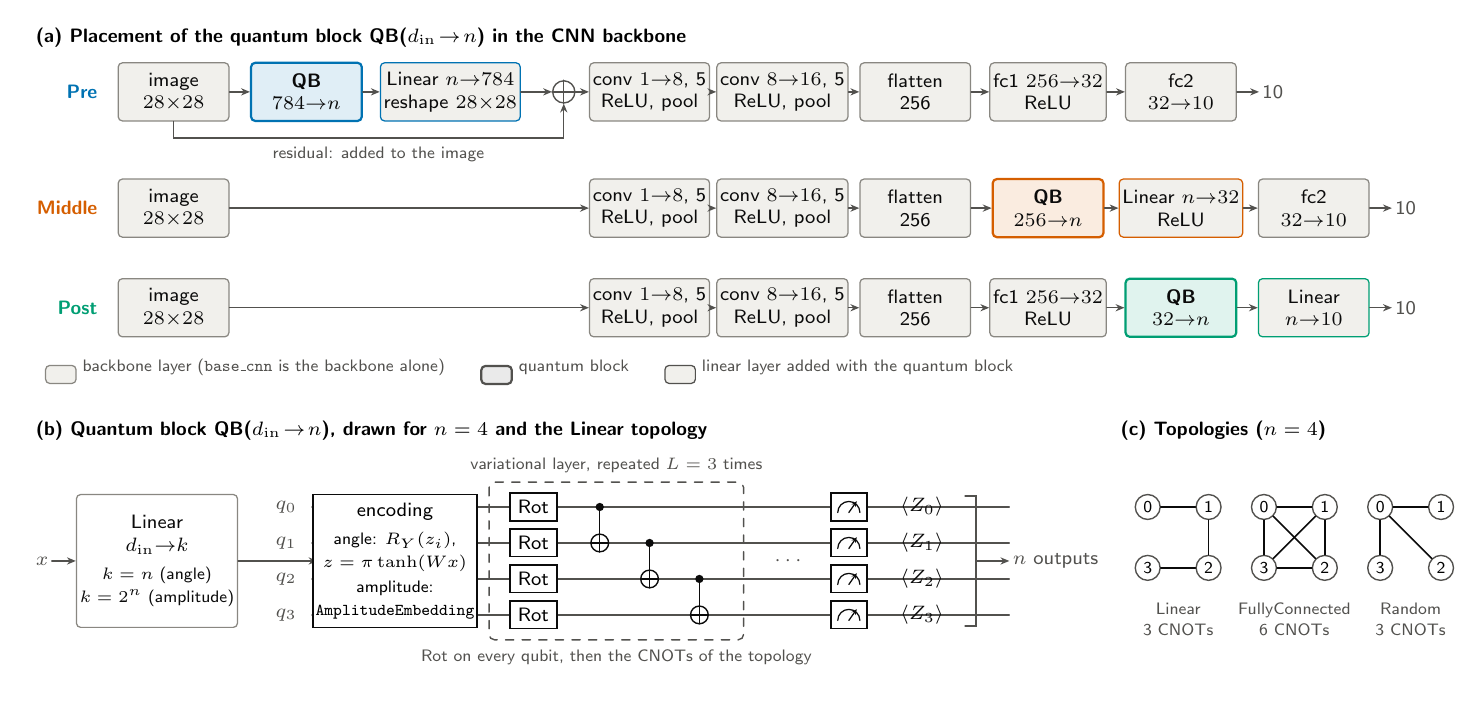
\begin{tikzpicture}[
    font=\fontsize{7}{8.2}\selectfont, line cap=round, >={Stealth[length=3.2pt,width=2.6pt]},
    box/.style={draw=clsline, fill=cls, rounded corners=1.5pt, line width=0.45pt, align=center,
                minimum width=40pt, minimum height=21pt, inner sep=1.2pt, text=ink},
    qb/.style={box, line width=0.8pt, font=\fontsize{7}{8.2}\selectfont\bfseries},
    arr/.style={->, line width=0.5pt, draw=ink2},
    rowlab/.style={font=\fontsize{7.5}{9}\selectfont\bfseries, anchor=east},
    wire/.style={line width=0.45pt, draw=ink2},
    gate/.style={draw=ink, fill=white, line width=0.5pt, minimum width=17pt, minimum height=10pt,
                 inner sep=0.8pt},
    panel/.style={font=\fontsize{7.5}{9}\selectfont\bfseries, anchor=south west, inner sep=0pt},
    note/.style={text=ink2, font=\fontsize{6.5}{7.6}\selectfont},
  ]

  % ---------------------------------------------------------------- (a) column positions (pt)
  \def\xIN{0pt}  \def\xQA{48pt} \def\xQB{100pt} \def\xADD{141pt} \def\xCa{172pt} \def\xCb{220pt}
  \def\xFL{268pt} \def\xHa{316pt} \def\xHb{364pt} \def\xHc{412pt}
  \def\yPre{0pt} \def\yMid{-42pt} \def\yPost{-78pt}

  \node[panel] at (-50pt, 16pt) {(a) Placement of the quantum block QB($d_{\mathrm{in}}\!\to\! n$) in the CNN backbone};

  % Pre
  \node[rowlab, text=pre] at (-24pt, \yPre) {Pre};
  \node[box] (pIN) at (\xIN, \yPre) {image\\$28\by28$};
  \node[qb, draw=pre, fill=pre!12] (pQ) at (\xQA, \yPre) {QB\\$784\ra n$};
  \node[box, draw=pre] (pL) at (\xQB, \yPre) {Linear $n\ra784$\\reshape $28\by28$};
  \node[circle, draw=ink2, line width=0.5pt, inner sep=0pt, minimum size=8pt] (pADD) at (\xADD, \yPre) {};
  \draw[line width=0.5pt, draw=ink2] (pADD.north) -- (pADD.south) (pADD.west) -- (pADD.east);
  \node[box] (pC1) at (\xCa, \yPre) {conv $1\ra8$, 5\\ReLU, pool};
  \node[box] (pC2) at (\xCb, \yPre) {conv $8\ra16$, 5\\ReLU, pool};
  \node[box] (pFL) at (\xFL, \yPre) {flatten\\256};
  \node[box] (pF1) at (\xHa, \yPre) {fc1 $256\ra32$\\ReLU};
  \node[box] (pF2) at (\xHb, \yPre) {fc2\\$32\ra10$};
  \draw[arr] (pIN) -- (pQ); \draw[arr] (pQ) -- (pL); \draw[arr] (pL) -- (pADD); \draw[arr] (pADD) -- (pC1);
  \draw[arr] (pC1) -- (pC2); \draw[arr] (pC2) -- (pFL); \draw[arr] (pFL) -- (pF1); \draw[arr] (pF1) -- (pF2);
  \draw[arr] (pIN.south) -- ++(0, -6pt) -| (pADD.south);
  \node[note, anchor=north] at ($(\xQA, \yPre)!0.5!(\xQB, \yPre) + (0, -16.5pt)$) {residual: added to the image};

  % Middle
  \node[rowlab, text=mid] at (-24pt, \yMid) {Middle};
  \node[box] (mIN) at (\xIN, \yMid) {image\\$28\by28$};
  \node[box] (mC1) at (\xCa, \yMid) {conv $1\ra8$, 5\\ReLU, pool};
  \node[box] (mC2) at (\xCb, \yMid) {conv $8\ra16$, 5\\ReLU, pool};
  \node[box] (mFL) at (\xFL, \yMid) {flatten\\256};
  \node[qb, draw=mid, fill=mid!12] (mQ) at (\xHa, \yMid) {QB\\$256\ra n$};
  \node[box, draw=mid] (mL) at (\xHb, \yMid) {Linear $n\ra32$\\ReLU};
  \node[box] (mF2) at (\xHc, \yMid) {fc2\\$32\ra10$};
  \draw[arr] (mIN) -- (mC1); \draw[arr] (mC1) -- (mC2); \draw[arr] (mC2) -- (mFL); \draw[arr] (mFL) -- (mQ);
  \draw[arr] (mQ) -- (mL); \draw[arr] (mL) -- (mF2);

  % Post
  \node[rowlab, text=post] at (-24pt, \yPost) {Post};
  \node[box] (qIN) at (\xIN, \yPost) {image\\$28\by28$};
  \node[box] (qC1) at (\xCa, \yPost) {conv $1\ra8$, 5\\ReLU, pool};
  \node[box] (qC2) at (\xCb, \yPost) {conv $8\ra16$, 5\\ReLU, pool};
  \node[box] (qFL) at (\xFL, \yPost) {flatten\\256};
  \node[box] (qF1) at (\xHa, \yPost) {fc1 $256\ra32$\\ReLU};
  \node[qb, draw=post, fill=post!12] (qQ) at (\xHb, \yPost) {QB\\$32\ra n$};
  \node[box, draw=post] (qL) at (\xHc, \yPost) {Linear\\$n\ra10$};
  \draw[arr] (qIN) -- (qC1); \draw[arr] (qC1) -- (qC2); \draw[arr] (qC2) -- (qFL); \draw[arr] (qFL) -- (qF1);
  \draw[arr] (qF1) -- (qQ); \draw[arr] (qQ) -- (qL);

  % class scores
  \foreach \n in {pF2, mF2, qL} { \draw[arr] (\n.east) -- ++(8pt, 0) node[right, inner sep=1pt, text=ink2] {10}; }

  % legend for (a)
  \node[note, anchor=north west] at (-50pt, \yPost - 15pt)
    {\tikz[baseline=-2.4pt]\node[box, minimum width=11pt, minimum height=6.5pt]{};\ backbone layer (\texttt{base\_cnn} is the backbone alone)\qquad
     \tikz[baseline=-2.4pt]\node[box, line width=0.8pt, draw=ink2, fill=ink2!12, minimum width=11pt, minimum height=6.5pt]{};\ quantum block\qquad
     \tikz[baseline=-2.4pt]\node[box, draw=ink2, minimum width=11pt, minimum height=6.5pt]{};\ linear layer added with the quantum block};

  % ---------------------------------------------------------------- (b) quantum block, n = 4
  \begin{scope}[yshift=-150pt]
    \node[panel] at (-50pt, 24pt) {(b) Quantum block QB($d_{\mathrm{in}}\!\to\! n$), drawn for $n = 4$ and the Linear topology};
    \def\dy{13pt}
    \foreach \q in {0,1,2,3} {
      \draw[wire] (50pt, -\q*\dy) -- (302pt, -\q*\dy);
      \node[anchor=east, text=ink2] at (48pt, -\q*\dy) {$q_{\q}$};
    }
    \node[box, fill=white, minimum width=44pt, minimum height=48pt] (inx) at (-6pt, -1.5*\dy)
      {Linear\\$d_{\mathrm{in}}\ra k$\\[2pt]{\fontsize{6}{7}\selectfont $k = n$ (angle)}\\{\fontsize{6}{7}\selectfont $k = 2^n$ (amplitude)}};
    \draw[arr] (-44pt, -1.5*\dy) -- (inx.west) node[pos=0, left, inner sep=1pt, text=ink2] {$x$};
    \draw[arr] (inx.east) -- (52pt, -1.5*\dy);
    \node[draw=ink, fill=white, line width=0.5pt, minimum width=50pt, minimum height=48pt, align=center,
          inner sep=1pt] (enc) at (80pt, -1.5*\dy)
      {encoding\\[2pt]{\fontsize{6}{7}\selectfont angle: $R_Y(z_i)$,}\\{\fontsize{6}{7}\selectfont $z=\pi\tanh(Wx)$}\\[1pt]{\fontsize{6}{7}\selectfont amplitude:}\\{\fontsize{6}{7}\selectfont\texttt{AmplitudeEmbedding}}};
    % one variational layer (repeated L = 3 times)
    \foreach \q in {0,1,2,3} { \node[gate] at (130pt, -\q*\dy) {Rot}; }
    \foreach \c/\t/\x in {0/1/154, 1/2/172, 2/3/190} {
      \fill[ink] (\x pt, -\c*\dy) circle (1.5pt);
      \draw[line width=0.5pt, draw=ink] (\x pt, -\c*\dy) -- (\x pt, -\t*\dy - 3.2pt);
      \draw[line width=0.5pt, draw=ink, fill=white] (\x pt, -\t*\dy) circle (3.2pt);
      \draw[line width=0.5pt, draw=ink] (\x pt - 3.2pt, -\t*\dy) -- (\x pt + 3.2pt, -\t*\dy)
                                        (\x pt, -\t*\dy + 3.2pt) -- (\x pt, -\t*\dy - 3.2pt);
    }
    \draw[dashed, line width=0.5pt, draw=ink2, rounded corners=2pt] (114pt, 9pt) rectangle (206pt, -3*\dy - 9pt);
    \node[note, anchor=south] at (160pt, 9pt) {variational layer, repeated $L = 3$ times};
    \node[note, anchor=north] at (160pt, -3*\dy - 9pt) {Rot on every qubit, then the CNOTs of the topology};
    \node[text=ink2] at (222pt, -1.5*\dy) {$\cdots$};
    % measurement
    \foreach \q in {0,1,2,3} {
      \node[gate, minimum width=13pt] (m\q) at (244pt, -\q*\dy) {};
      \draw[line width=0.45pt, draw=ink] ($(m\q.center)+(-4pt,-2pt)$) arc (180:0:4pt);
      \draw[line width=0.45pt, draw=ink, ->, >={Stealth[length=2pt,width=1.8pt]}] ($(m\q.center)+(0,-2pt)$) -- ++(55:5pt);
      \node[anchor=west, text=ink] at (259pt, -\q*\dy) {$\langle Z_{\q}\rangle$};
    }
    \draw[line width=0.5pt, draw=ink2] (286pt, 4pt) -- (290pt, 4pt) -- (290pt, -3*\dy - 4pt) -- (286pt, -3*\dy - 4pt);
    \draw[arr] (290pt, -1.5*\dy) -- (302pt, -1.5*\dy) node[right, inner sep=1pt, text=ink2] {$n$ outputs};
  \end{scope}

  % ---------------------------------------------------------------- (c) topologies, n = 4
  \begin{scope}[xshift=352pt, yshift=-150pt]
    \node[panel] at (-10pt, 24pt) {(c) Topologies ($n = 4$)};
    \tikzset{qn/.style={circle, draw=ink2, fill=white, line width=0.5pt, inner sep=0pt, minimum size=9pt,
                        font=\fontsize{6}{7}\selectfont}}
    \foreach \name/\x/\edges/\lab/\cnt in {
        lin/0/{0/1,1/2,2/3}/Linear/{3},
        fc/42/{0/1,0/2,0/3,1/2,1/3,2/3}/FullyConnected/{6},
        rnd/84/{0/1,0/2,0/3}/Random/{3}} {
      \begin{scope}[xshift=\x pt]
        \node[qn] (\name0) at (0pt, 0pt) {0};    \node[qn] (\name1) at (22pt, 0pt) {1};
        \node[qn] (\name2) at (22pt, -22pt) {2}; \node[qn] (\name3) at (0pt, -22pt) {3};
        \foreach \a/\b in \edges { \draw[line width=0.6pt, draw=ink] (\name\a) -- (\name\b); }
        \node[note, anchor=north, align=center] at (11pt, -31pt) {\lab\\\cnt\ CNOTs};
      \end{scope}
    }
  \end{scope}
\end{tikzpicture}
\end{document}
